\documentclass[11pt, a4paper]{scrartcl}
\usepackage{graphicx}
\usepackage{color}
\begin{document}

%Alles zu UproC
\section{UproC}

\subsection{UproC Ausgabe}
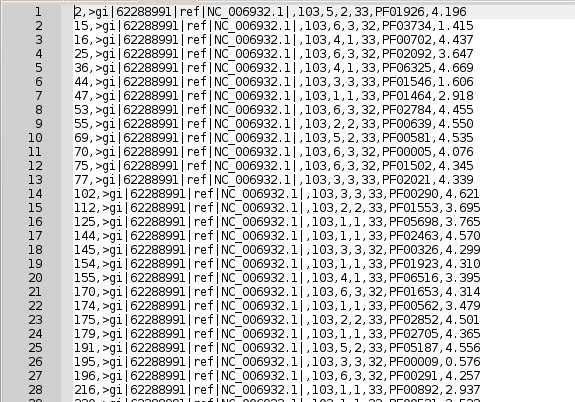
\includegraphics[width=0.7\textwidth]{/work/gi/studprj/metaclassify/UproC/snapshot_output_uproc.png}
\linebreak

\subsection{Beschreibung der Ausgabe}
\begin{flushleft}
\textbf{1.} sequence number\linebreak
\textbf{2.} sequence header up to the first white space\linebreak
\textbf{3.} sequence length\linebreak
\textbf{4.} ORF-frame (1-6)\linebreak
\textbf{5.} ORF index in the sequence (starting with 1)\linebreak
\textbf{6.} ORF length\linebreak
\textbf{7.} predicted protein family\linebreak
\textbf{8.} classification score
\linebreak\linebreak
ORF = open reading frame
\end{flushleft}
\newpage

%Alles zu Diamond
\section{Diamond}

\subsection{Diamond Ausgabe}
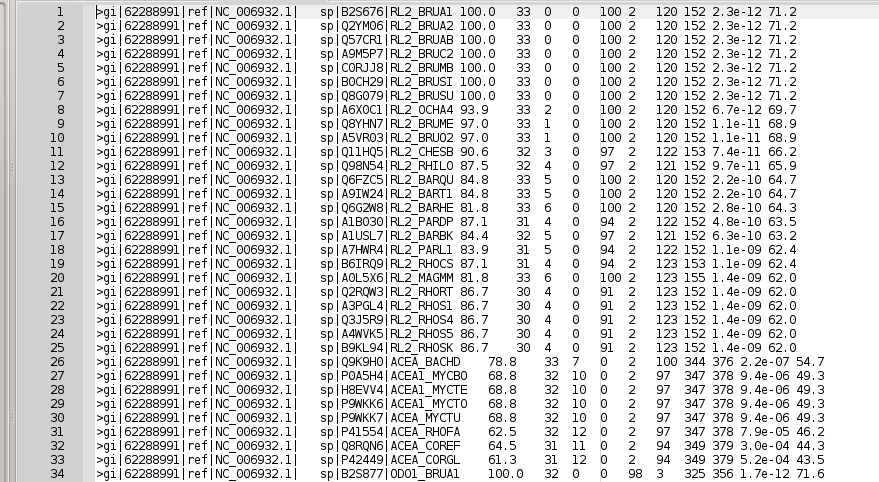
\includegraphics[width=0.7\textwidth]{/work/gi/studprj/metaclassify/Diamond/snapshot1_output_diamond.png}

\subsection{Beschreibung der Ausgabe}
\begin{flushleft}
\textbf{1.} query seq-ID\linebreak
\textbf{2.} subject seq-ID\linebreak
\textbf{3.} percentage of identical matches\linebreak
\textbf{4.} length of alignment\linebreak
\textbf{5.} number of missmatches\linebreak
\textbf{6.} number of gap openings\linebreak
\textbf{7.} start of alignment in query\linebreak
\textbf{8.} end of alignment in query\linebreak
\textbf{9.} start of alignment in subject\linebreak
\textbf{10.} end of alignment in subject\linebreak
\textbf{11.} e-value\linebreak
\textbf{12.} bit-score
\end{flushleft}
\newpage

%Alles zu Lambda
\section{Lambda}

\subsection{Lambda Ausgabe}
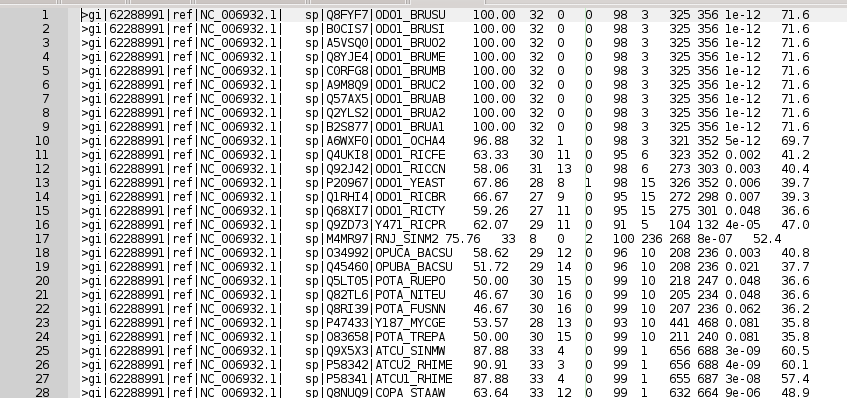
\includegraphics[width=0.7\textwidth]{/work/gi/studprj/metaclassify/Lambda/snapshot2_output_lambda.png}

\subsection{Beschreibung der Ausgabe}
\begin{flushleft}
\textbf{1.} query seq-ID\linebreak
\textbf{2.} subject seq-ID\linebreak
\textbf{3.} percentage of identical matches\linebreak
\textbf{4.} length of alignment\linebreak
\textbf{5.} number of missmatches\linebreak
\textbf{6.} number of gap openings\linebreak
\textbf{7.} start of alignment in query\linebreak
\textbf{8.} end of alignment in query\linebreak
\textbf{9.} start of alignment in subject\linebreak
\textbf{10.} end of alignment in subject\linebreak
\textbf{11.} e-value\linebreak
\textbf{12.} bit-score
\end{flushleft}

\section{Vergleich}

Lamdba und Diamond stimmen in Ausgaben ueberein. UproC unterscheidet sich deutlich in dem was ausgegeben wird --$>$ kein Bezug auf die Vergleichssequenz.


\end{document}

